\begin{itemize}
	\item \textbf{Meeting Document}

\begin{itemize} 
\item[$\circ$] After the Monday operations meeting, an OOD or any operator assigned by the OOD should open new operations meeting minutes for the week. 
\item[$\circ$] Ensure that you copy the template from the 2021 Operations meetings and verify that the new copy is saved in the new folder.
\item[$\circ$] The name of the document is the current Monday date to the following Monday date as in \textbf{Figure}~\ref{fig:image86}.
\end{itemize}
\begin{figure}[!thb]
	\centering
	%\includegraphicsdpi{100}{}{bur1.png}     
	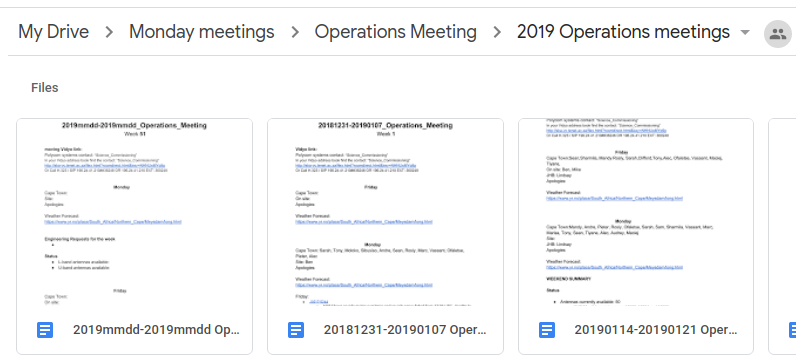
\includegraphics[scale=0.53]{Chapters/images/image86.png}
	
	%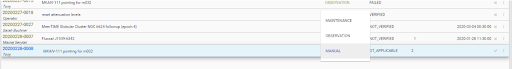
\includegraphics[resolution=100]{bur1.png}
	\caption{Operations meeting document google folder}
	\label{fig:image86}
\end{figure}


\item \textbf{Status}
\begin{itemize} 
\item[$\circ$] How many operational antennas are available currently in both bands L and UHF?
\item[$\circ$] How many antennas are currently in maintenance, today? Reason? When are they returning?

\item[$\circ$] Link each issue to a JIRA
\item[$\circ$] Always remember to report trends/frequencies of similar issues.
\item[$\circ$] Divide issues in each section by the days which they occured.
\end{itemize}
\item \textbf{CAM/SP/CBF}
\begin{itemize} 
\item[$\circ$] What are the latest changes/deployments/hot-fixes done this week?
\item[$\circ$] What are some of the issues experienced from CAM on the system, are they resolved? If not what is the current status of the problem?
\end{itemize}
\item \textbf{Digitisers/ Receivers and APs}
\begin{itemize} 
\item[$\circ$] Are there latest software/firmware updates done?
\item[$\circ$] Any other recent work done on each AP,dig or RSC?
\item[$\circ$] What are the issues on each APs? What did they affect? How long were they in erroneous state for? Has the JIRA been attended to? 
\item[$\circ$] What is the resolution if there is one? Is there a procedure from this JIRA? You can also choose to include some of this information under the observation session….. Where they are most relevant as to when they happened.
\end{itemize}
\item \textbf{Integration and Testing}
\begin{itemize} 
\item[$\circ$]Ensure that what you are reporting to have happened in the week actually has happened and perhaps on the Thursday or Friday morning ask the people responsible for that task for feedback for this meeting, they can fill it in themselves in the minutes if you do not understand the details.
\end{itemize}
\end{itemize}
\textbf{Notice Board}
If there are any issues that you will like other operators to be aware of please add to the electronic notice board at \url{https://docs.google.com/document/d/1YvHi7U63WUbkbUGOQRW\_PJcZZlRzpOYb6mnv2CZlkSM/edit}

